O Merge Sort é um algoritmo de ordenação bastante diferente do Insertion Sort, tanto em abordagem quanto em eficiência. Enquanto o Insertion Sort constrói a lista ordenada um item por vez, inserindo cada novo elemento em sua posição correta dentro da parte já ordenada, o Merge Sort adota uma estratégia de "dividir para conquistar"\cite{cyberini2018mergesort}.

 \begin{figure}[H]
    \centering
    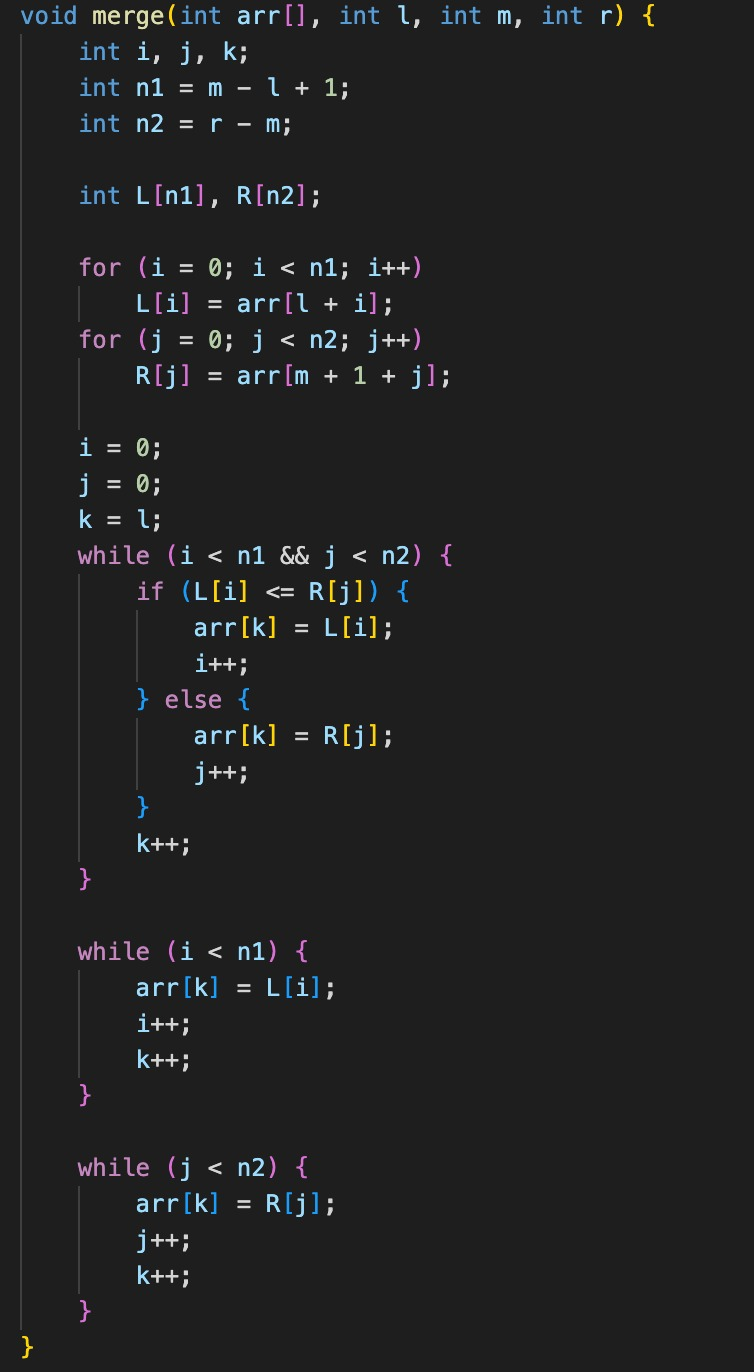
\includegraphics[width = 6cm]{Imagens/Merge Sort/WhatsApp Image 2023-11-13 at 21.41.34.jpeg}
    \caption{ALgoritmo Merge Sort, imagem criada pelo autor. }
    \label{imagem_merge}
\end{figure}

 \begin{figure}[H]
    \centering
    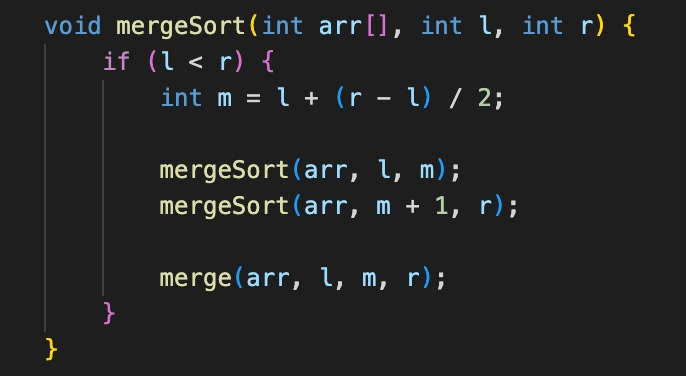
\includegraphics[width = 6cm]{Imagens/Merge Sort/WhatsApp Image 2023-11-13 at 21.41.34 (1).jpeg}
    \caption{ALgoritmo Merge Sort, imagem criada pelo autor. }
    \label{imagem_merge}
\end{figure}

\par A seguir, um exemplo do funcionamento do Merge Sort:

 \begin{figure}[H]
    \centering
    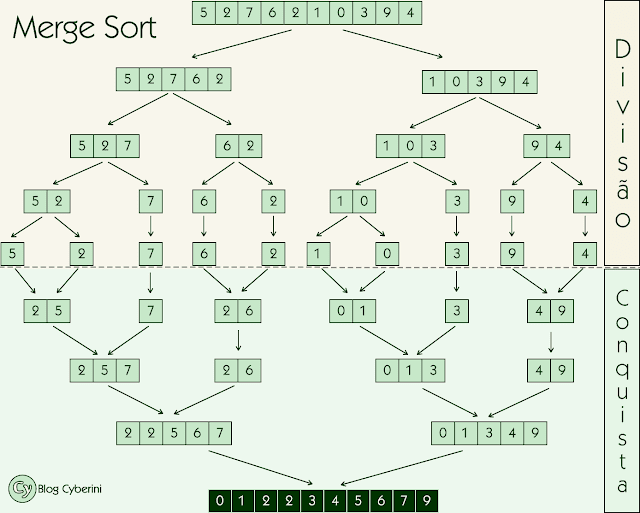
\includegraphics[width = 6cm]{Imagens/Merge Sort/diagrama-merge-sort.png}
    \caption{Exemplo do Merge Sort\cite{cyberini2018mergesort}. }
    \label{imagem_digrama}
\end{figure}

Como mostrado na Figura~\ref{fig:imagem_diagrama}, o Merge Sort funciona da seguinte maneira: 
1-Divisão Recursiva: O Merge Sort começa dividindo o conjunto de dados em duas metades iguais (ou quase iguais). Essa divisão continua recursivamente até que cada subconjunto contenha apenas um elemento (ou nenhum, se o conjunto inicial for vazio).

2-Fusão e Ordenação: Após a divisão, o algoritmo começa a combinar os subconjuntos, ordenando-os no processo. Dois subconjuntos são comparados elemento a elemento, e os elementos são ordenados e mesclados em um novo subconjunto. Esse processo de fusão continua até que todos os subconjuntos pequenos sejam combinados de volta em um único conjunto ordenado.
